%% Hanford investigations

%% TCS schematic for LIGO Hanford for O3
%% TCS pre-loading
 %% Current methodology for tuning TCS
  %% Detail Hanford's methods
 %% Increasing RH tuning speed


%As shown in Chapter 1,  increasing input power leads to a direct increase to the sensitivity of a DRFPMI to make gravitational wave detections. But one implication of this is the necessity for thermal compensation. As the interferometer increases input power, you directly couple more light into the Fabry-P\'{e}rot cavity arms; and even with optics ultra-low absorption ($\approx 400 \; \mathrm{ppb} \pm 150 \; \mathrm{ppb}$ \textcolor{red}{alog ? or point absorber paper}) still induce thermo-optic effects with the projected circulating arm power of 200 kW. A symptom of this is mode mismatch throughout the interferometer, a problem that contributes to loss of usable optical power throughought the DRFPMI which can reduce sensitivity two-fold: loss of power to your readout, and reduced efficacy of the current solution to reduce the quantum noise limit (squeezing).

During O3a the LIGO Hanford observatory circulating arm power reached beyond 180 kW; emphasizing importance on properly tuned thermal compensation in O3 to avert arm cavity mode mismatch. Detailed in this chapter is a summary of related comissioning efforts at LHO including but not exclusive to: citations of the initial computed O3 TCS pre-load, the development and implementation of real-time digital filtering for an improved ring heater actuation response by a factor of $\approx 6$, and the impacts of high absorption points aka point absorbers discovered on arm cavity test masses along with the inital efforts to mitigate them. 

\section{A priori TCS pre-load methodology for O3a}
Preserving arm cavity resonances requires countering the positive thermal lens defocus of the nominal test mass lens induced by high circulating interferometer arm cavity power. Preparing for this central uniform test mass distortion from the carrier beam requires calibrated and well established thermal actuator settings which in turn informs how much to `pre-load' the TCS actuators using early estimates of test mass absorption. Initial order of magnitude estimates of wavefront distortion from ultra-low absorption fused silica test masses under the influence of a centered high power gaussian beam as well as annular ring heater actuation are available \cite{hellovinet, Ramette:16}; though variations of the absorption between any two test mass mirrors are accounted for through calibrated defocus measurements using the Hartmann wavefront sensors sensitive to auxilary beams imaged onto the test mass mirror surfaces. Measured wavefront distortion is then mapped in real time to Zernike polynomial coefficients used to compute a differential defocus in diopters.

\subsection{The thermo-optic response}
\begin{figure}[!ht]
  \centering
  \begin{subcaptiongroup}
	  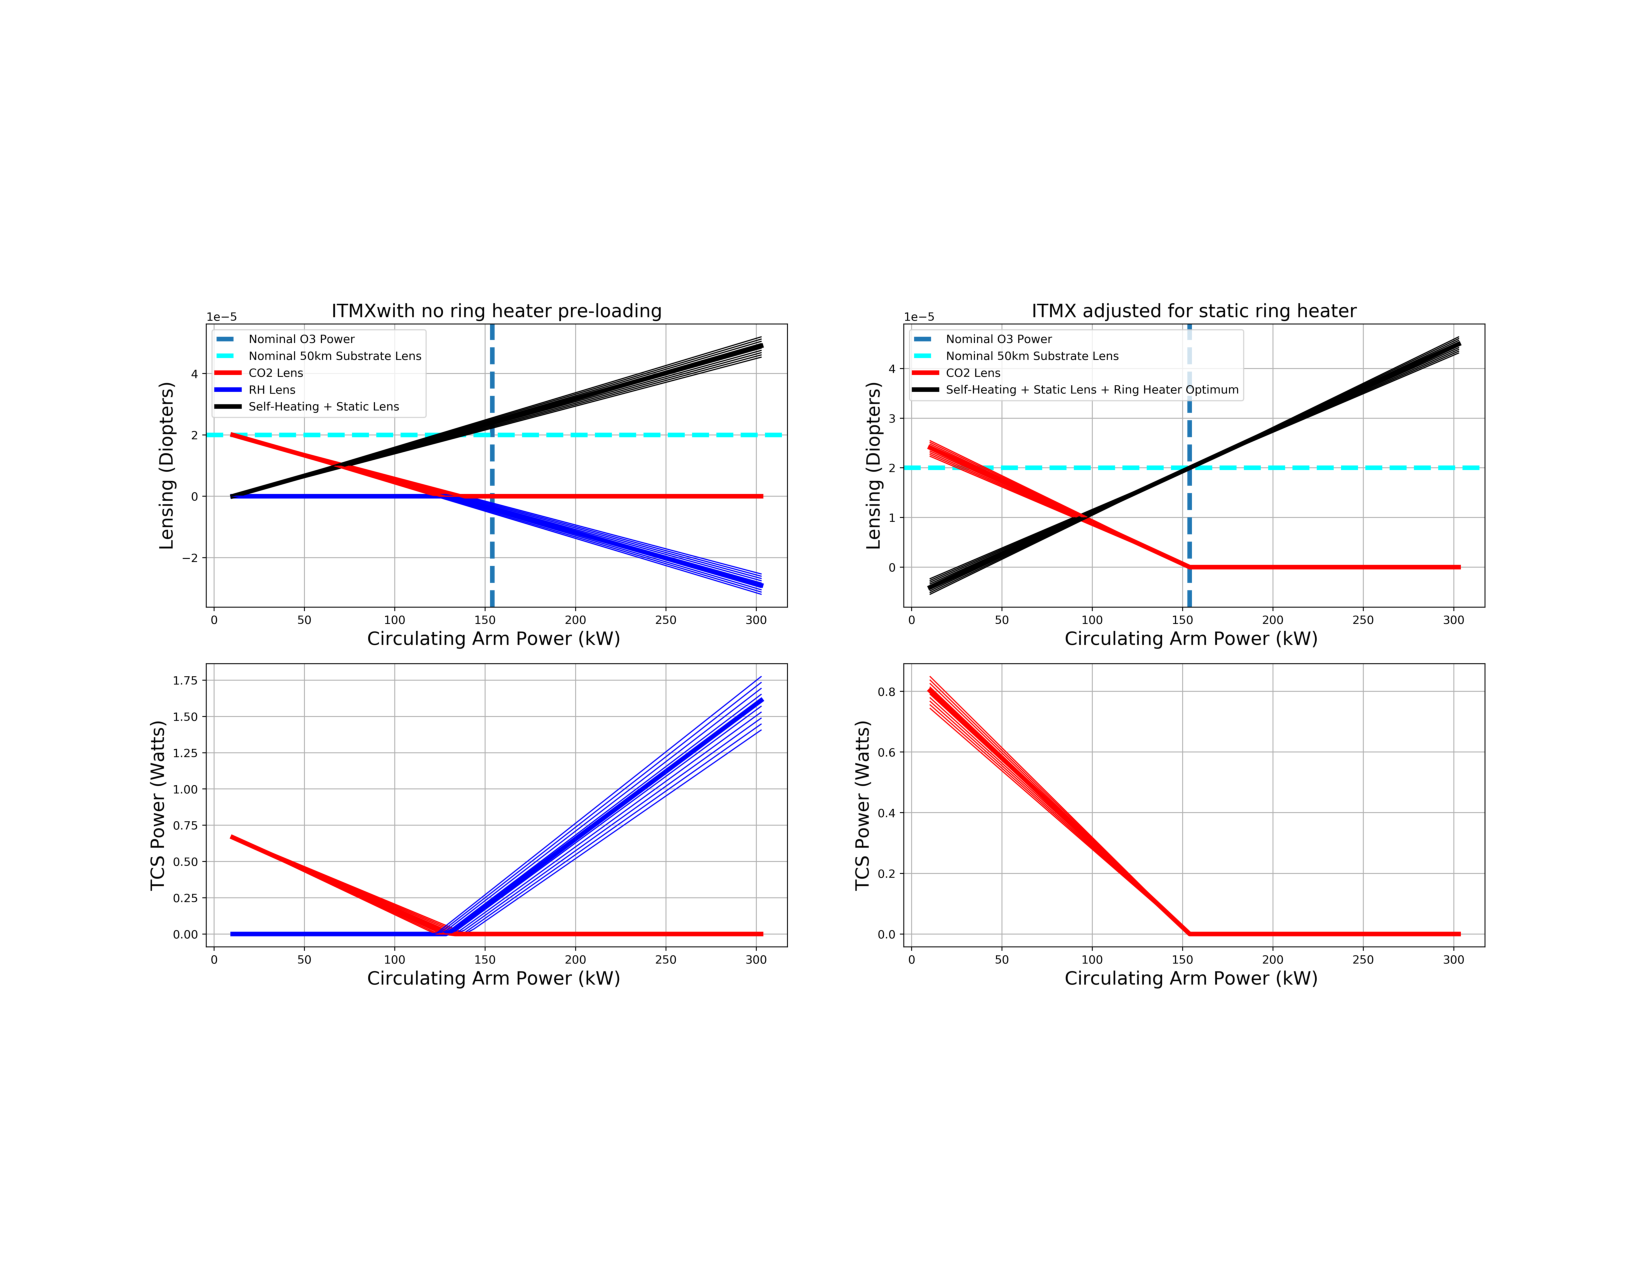
\includegraphics[width=\textwidth]{TCS/ITMX_TCS_Settings_tvo.pdf}
	  \phantomcaption\label{TO_response}
  \end{subcaptiongroup}
  \captionsetup{subrefformat=parens}
  \hfill
  \caption{Measured defocus from the carrier beam self heating and TCS actuation (central CO2 laser heating and annular ring heating.)} 
\label{fig:thermooptic_response}
\end{figure}
The thermo-optic time constant for the central self-heating response is quite similar to that seen from CO2 central actuation, though demonstrably different from annular ring heating. Because of this, LHO applies the central CO2 heating and static annular ring heating to a power level that respectively mimics and actuates for projected thermal deformation from the high power circulating resonant carrier beam in the Fabry-Perot arm cavities. Once the DRFPMI coupled cavities are configured or ``locked'', the input carrier power is gradually increased while CO2 laser powersimultaneously decreased in order to mitigate any possible differential thermo-optic response from the arm cavity test masses when reaching maximum power.
\begin{figure}[!ht]
  \centering
  \begin{subcaptiongroup}
	  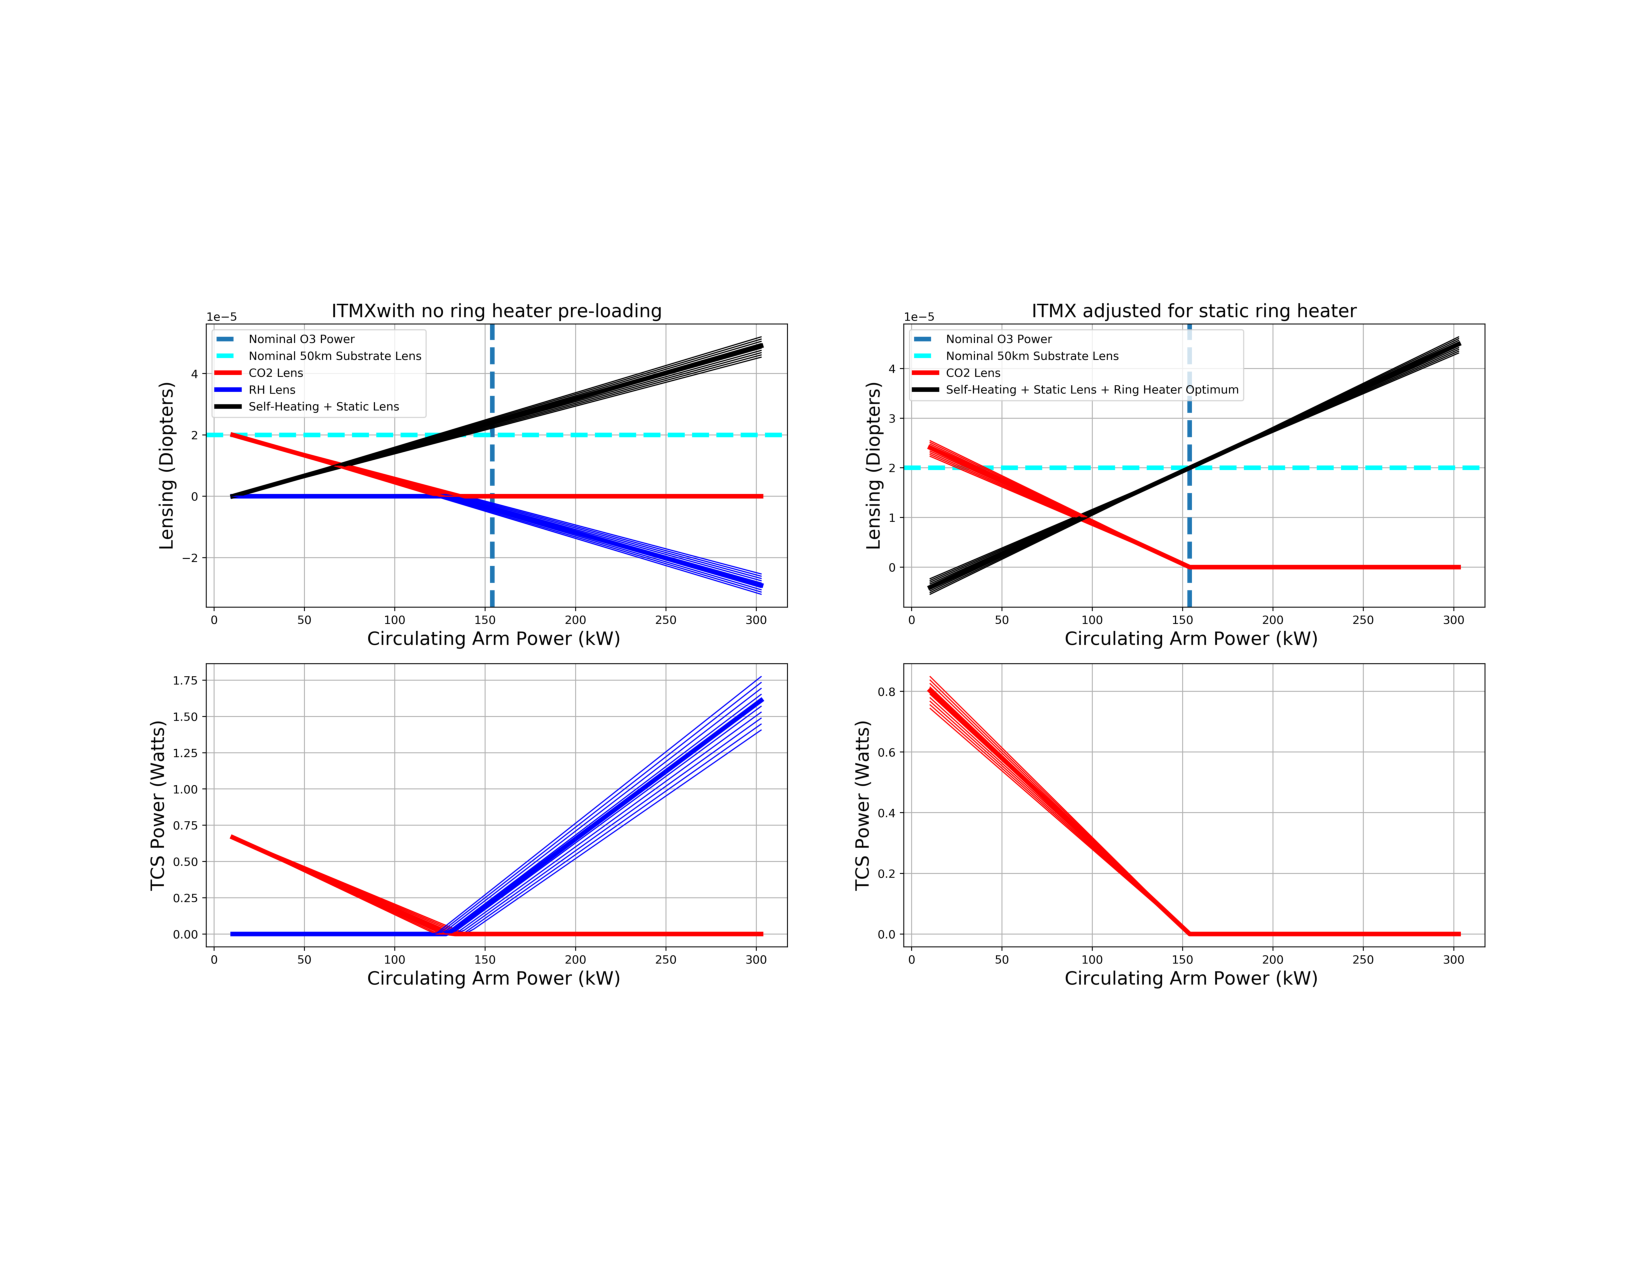
\includegraphics[width=\textwidth]{TCS/ITMX_TCS_Settings_tvo.pdf}
	  \phantomcaption\label{ITMX_TCS}
	  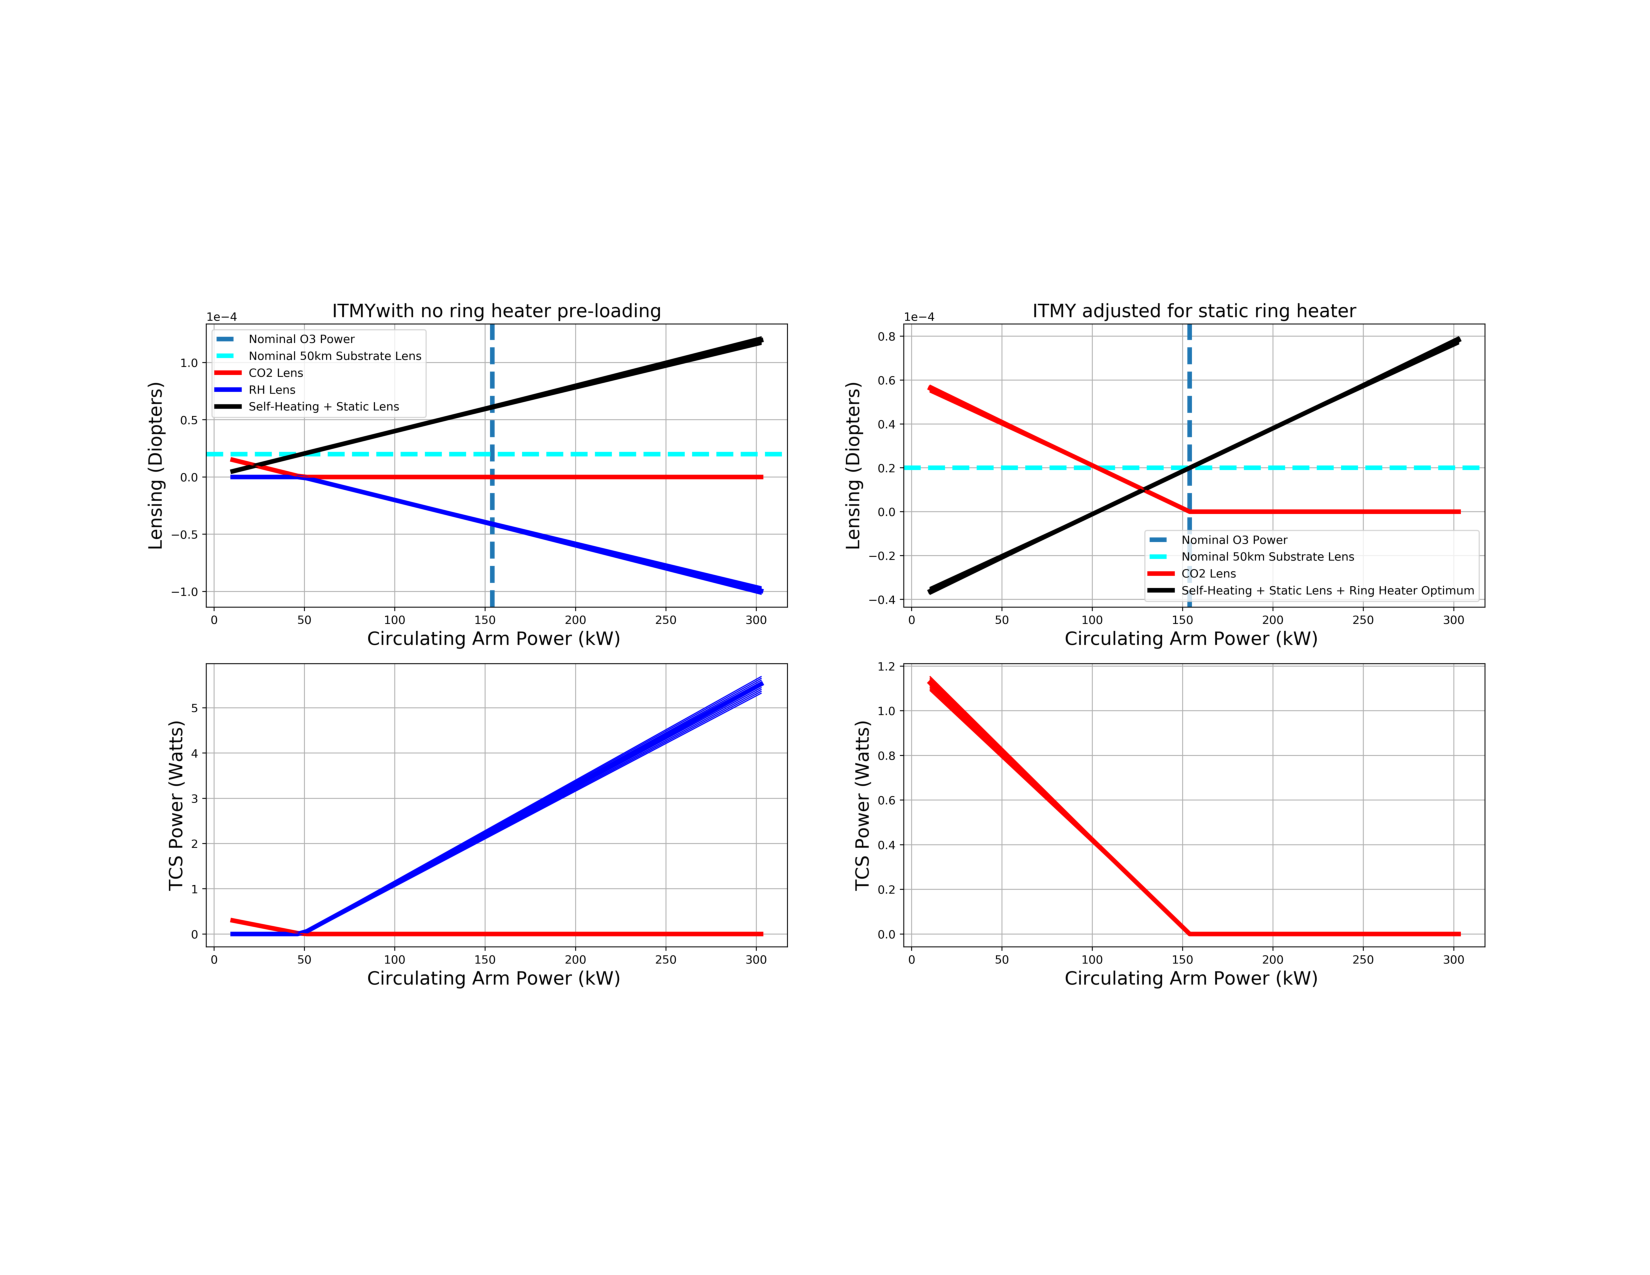
\includegraphics[width=\textwidth]{TCS/ITMY_TCS_Settings_tvo.pdf}
	  \phantomcaption\label{ITMY_TCS}
  \end{subcaptiongroup}
  \captionsetup{subrefformat=parens}
  \hfill
  \caption{The initial pre-load estimates for the ITMs at the LIGO Hanford Observatory for O3a as provided in \cite{tvo}} 
  \label{fig:O3_preload_tvo}
\end{figure}


\section{A posteriori thermal compensation for O3a}
While approaching designed arm cavity power, the presence of non-uniform absorption on the test mass coating surface imposed limits to reaching designed power and hence designed sensitivity; which simultaneously lead to a significant deviation from the original TCS pre-loading algorithm.  Assessment of these absorbers can inform methods of improving detector sensitivity required and initial characterization of these high absorbtion points which includes noting the characteristic optical path distortion as measured on the Hartmann wavefront sensors and the impacts on interferometer operations especially at high power. Current thermal actuation solutions are currently designed to control the TEM00 beam waist size and location though adjustments and modifications of current actuators was tried. This summary indicates that these absorbers may impose a barrier to maintaining high power in the arm cavities if no further proactive measures are not taken or are not sufficient to bypass detector symptoms; whether they are a result of preventable surface particulates or improved higher frequency.  

%The presence of high absorption points on the test masses (aka point absorbers) required adjustments to the TCS pre-load and various ring heater and CO2 settings were sampled. Part of this sampling lead to the development of a input ring heater filter allowing actuation to reach ? percent of the desired optical power within 2 hours compared to the 12 hour response pre-filter. Higher spatial frequency actuation in the form of a CO2 mask was also tried.

\subsection{Point absorbers in O3a}
\subsubsection{ITMY absorbers}
\begin{figure}[H]
  \centering
  \begin{subcaptiongroup}
	  \includegraphics[width=.495\textwidth]{TCS/PA/ITMY_absorbers.pdf}
	  \phantomcaption\label{itmxpa_justself}
	  \includegraphics[width=.495\textwidth]{TCS/PA/ITMY_self.pdf}
	  \phantomcaption\label{itmxpa_selfplusabs}
  \end{subcaptiongroup}
  \captionsetup{subrefformat=parens}
  \hfill
  \caption{An isometric view of uniform absorption vs point absorption of LHO ITMY}
  \label{fig:ITMY_pabs}
\end{figure}

\subsubsection{ETMX absorbers}
\begin{figure}[H]
  \centering
  \begin{subcaptiongroup}
	  \includegraphics[width=.49\textwidth]{TCS/PA/ETMX_absorber_short_heat.pdf}
	  \phantomcaption\label{etmxpa_justself}
	  \includegraphics[width=.49\textwidth]{TCS/PA/ETMX_absorber_full_heat.pdf}
	  \phantomcaption\label{etmxpa_selfplusabs}
  \end{subcaptiongroup}
  \captionsetup{subrefformat=parens}
  \hfill
  \caption{An isometric view of uniform absorption vs point absorption of LHO ETMX. The Hartmann probe beam experienced significant clipping on the baffle}
  \label{fig:ETMX_pabs}
\end{figure}
\textcolor{red}{A summary of the found absorbers \\
	* Insert optical path distortion photos (taken using Dan's software too) \\
		* ITMY absorbers \\
		* ETM absorbers \\
	* Reference Aidan's paper} \\

Impact on interferometer contrast and transmission / co-resonance of higher order modes

\subsubsection{Notable impacts}
A significant number of lockloss events during the comissioning period for O3A when increasing detector input power were a direct result of the slow degredation of select optical sideband powers used to maintain the delicate coupled cavity configuration. And while sustaining interferometer DC readout the arm cavity would generate higher order modes sustained by an Output Mode Cleaner resonance; contaminating the carrier field at the output photodiode.

%\begin{figure}[!ht]
%	\centering
%	\begin{subcaptiongroup}
%		\includegraphics[width=\textwidth]{}
%		\phantomcaption\label{

	* Controls schema review \\
		* Sensor schema \\
		* Optical sidebands (higher order beat signals) \\
	* Parasitic higher order modes \\
		* Visible higher order modes at the anti-symmetric port \\
A significant amount of optical loss as a result of losing sideband power is reported \\
	* Lockloss caused by reduced sideband power with interferometer thermalization \\

\subsubsection{Attempted symptom reduction}
The trivial solution of reducing the test mass non-uniformity was tried but exhibited noticable limitations with the available degrees of freedom. To restore the uniformity of the test mass surface, a custom mask was constructed with the intention of imaging a negative of the optical path distortion high absorption points onto the surface with the CO2 laser combined with a static ring heater offset. 

The installation location of the mask and size was established using the relevant propogation and imaging tensors applied to the CO2 actuation field while mitigation of the aforementioned impacts provided comissioners with the notable metrics of success.


\textcolor{red}{Results}
\\
The extremely strict alignment requirement introduced difficulties while attempting to fulfill the promise of restoring uniform absorption. And although the presence of the absorber symptoms show coorelation with their prominence at high power, their collective reduction proved not to be as straightfoward.
	
	* CO2 with enhanced focus on absorbers and ring heater actuation
		* Very narrow alignment requirement
		* Improvement metrics
			* Restoring sideband power	
	* Adjusting interferometer to OMC mode matching
		* Improvement metrics:
			* Reduced HOM content at detector output
			* Tracking dither line amplitudes

%\begin{figure}[H]
%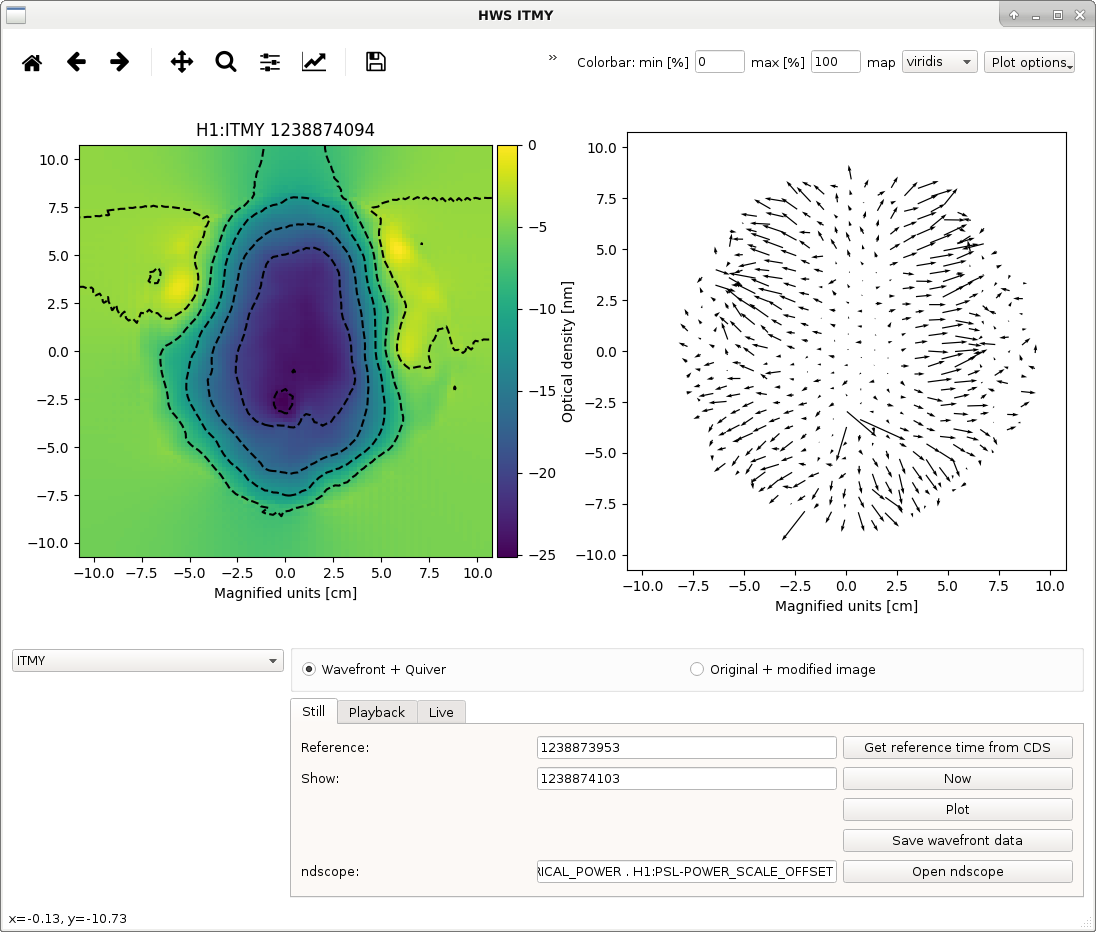
\includegraphics[width=\textwidth]{figs/TCS/PA/48349_20190409201649_inital_install_CO2Ymask2_150seconds_900mW.png}
%\caption{Point absorber figure with second $\mathrm{CO_2}$ mask}
%\label{fig:RH_power}
%\end{figure}

\section{Dynamic Thermal Compensation}
\subsection{A closer look at the ring heater / test mass thermo-optic response}
Transient ring heater actuation from a radially symmetric thermal aberration ($\Psi(t,r)$) is realized \cite{Ramette:16}:
\begin{equation}
	\Psi(t,r)=2\frac{dn}{dT} \sum^{\infty}_{m,p = 1} A_{m,p} \; c^{u}_{p} \mathrm{sin}(u_m h /2a) (a/u_m)[1-e^{-\alpha t}] J_0(\zeta_p r/a)
\end{equation}

\begin{figure}[H]
 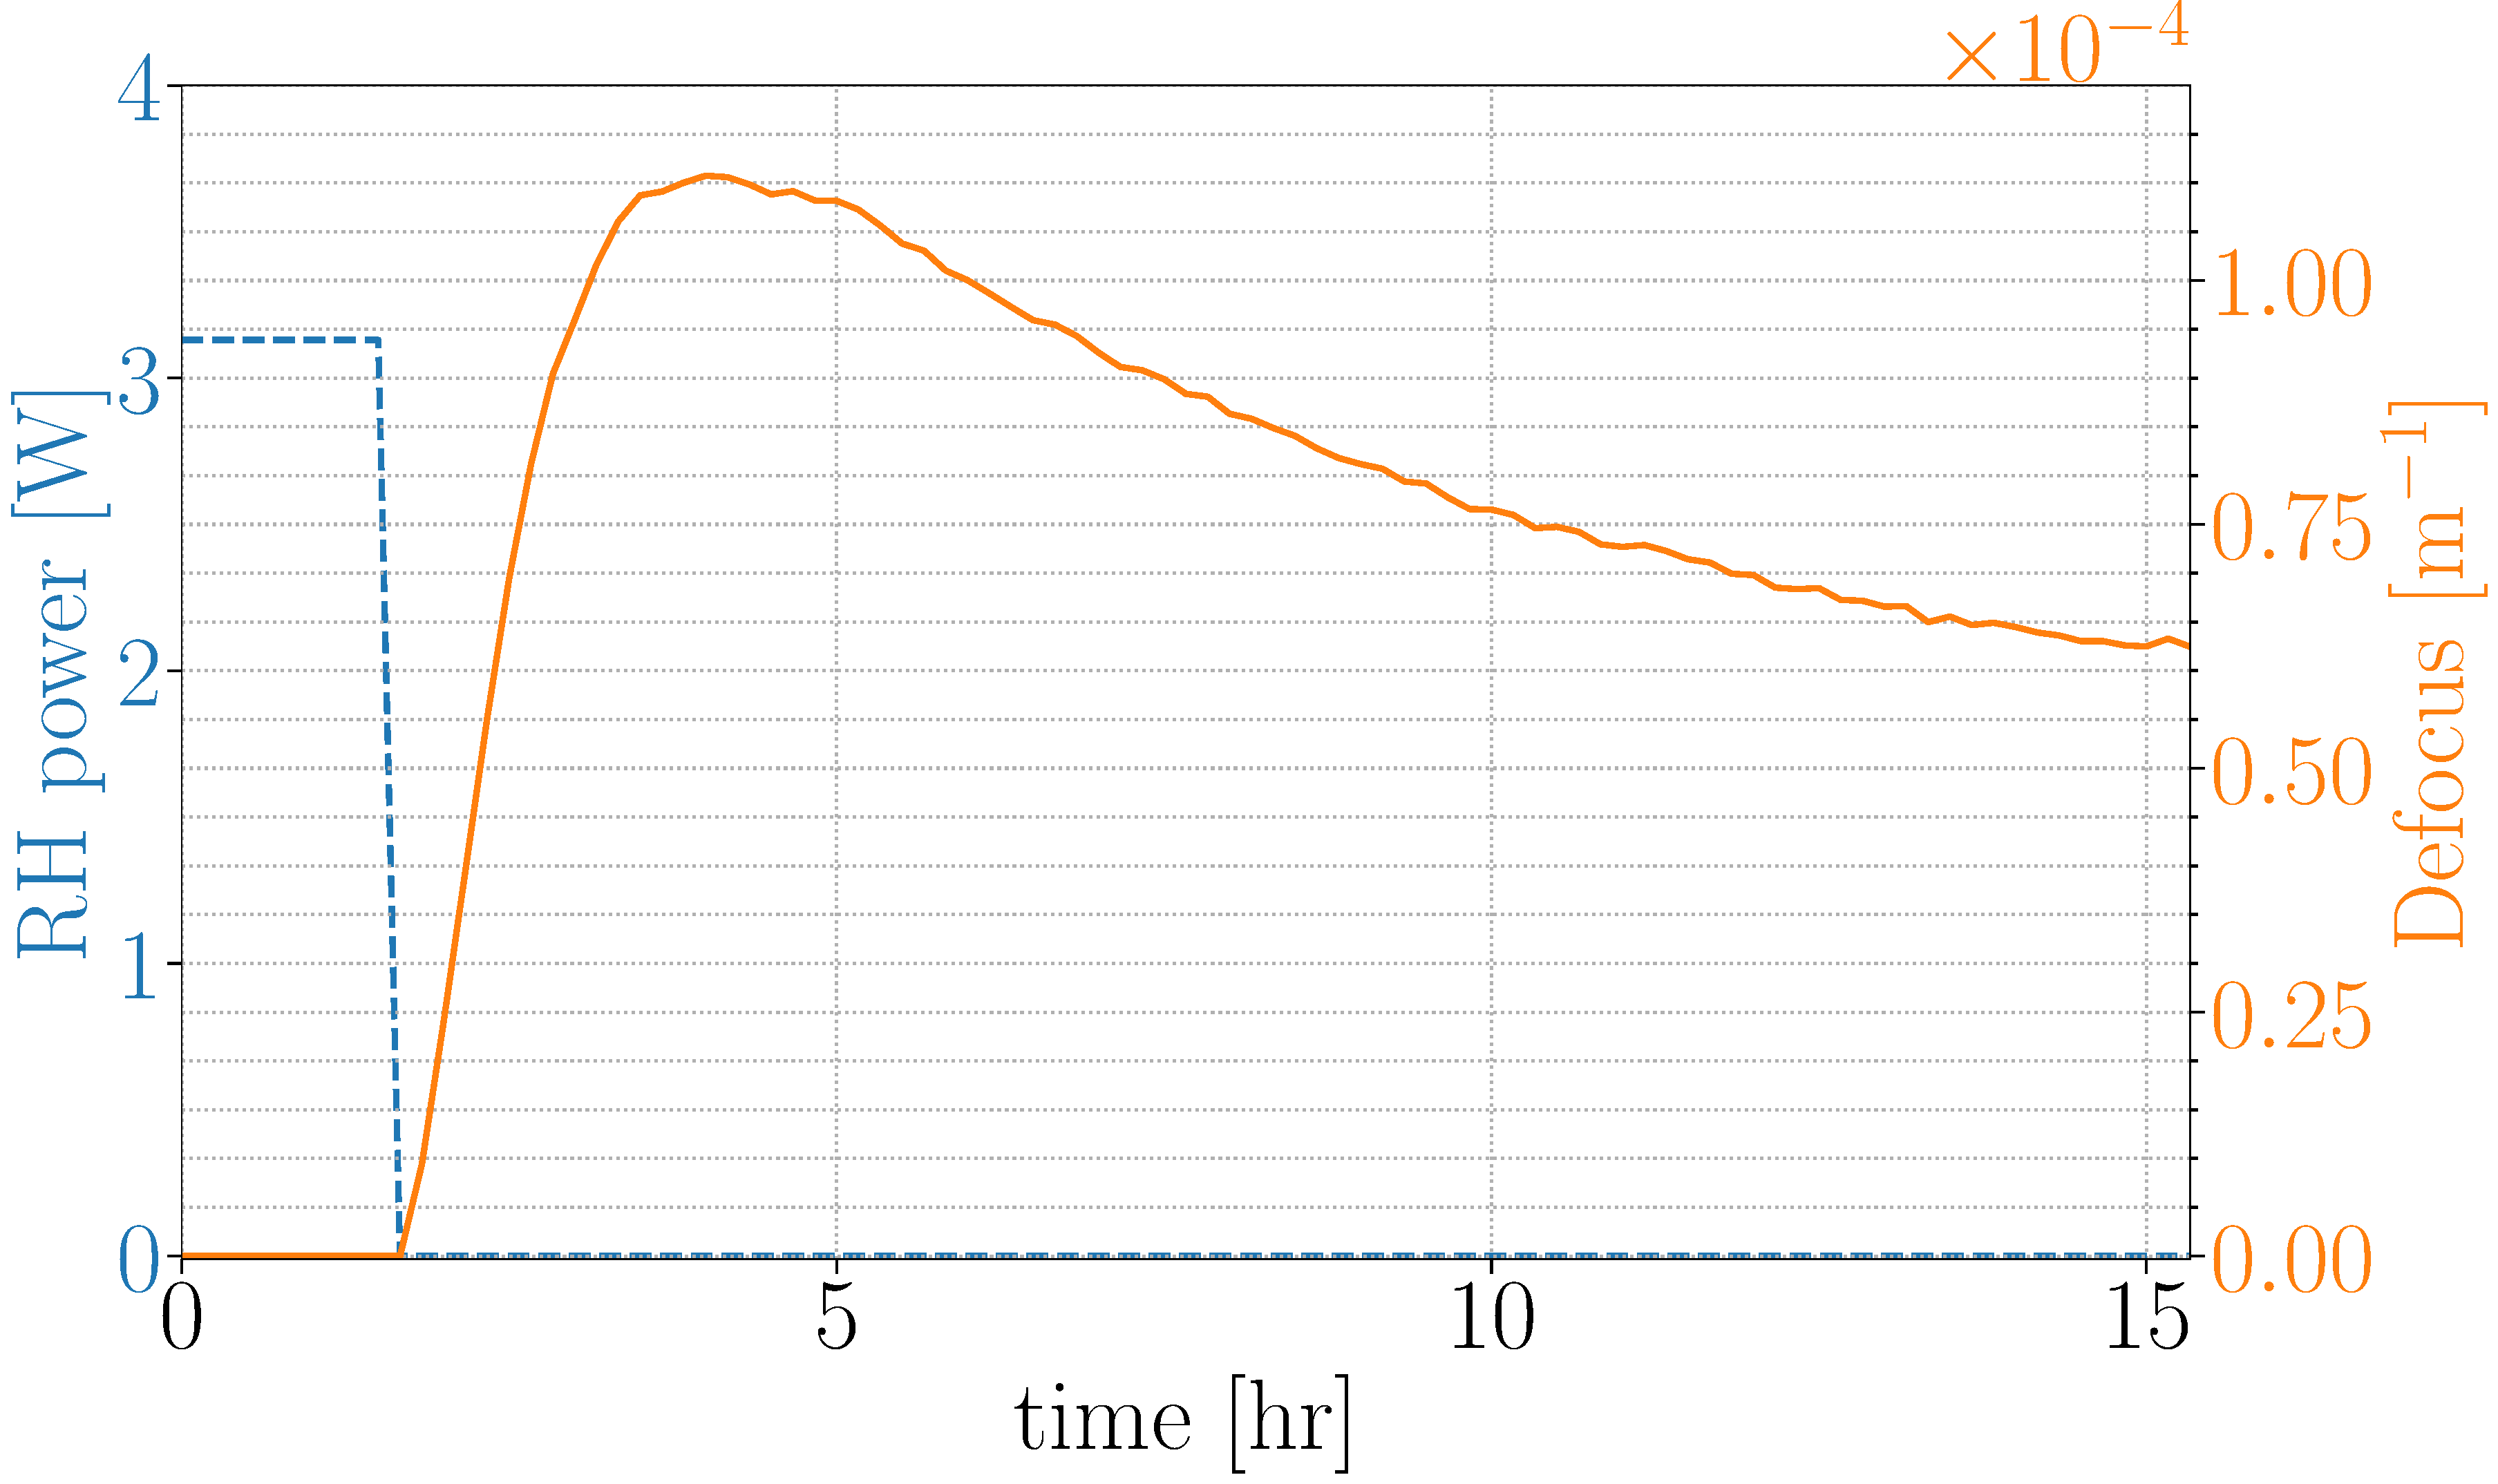
\includegraphics[width=\textwidth]{TCS/IRHF/Meas_response}
 \caption{ITMY thermo-optic response to a 3.13 [W] combined power reduction to the top and bottom ring heater elements. It's after $\approx$ 12 hours after the ring heater power control step do you start to see a small enough steady state differential defocus ($\frac{\mathrm{d} \alpha_\mathrm{sp}}{\mathrm{dt}}$) and can assume a steady state thermal lens.}
 \label{fig:RHresp}
\end{figure}

The measured thermo-optic step response exhibits differential defocusing for $\approx$ 12 to 15 hours once the ring heater power has been changed; and with a large enough power steps, these adjustments to ring heater power can significantly stall precious detector observing/comissioning time from the differential mode matching conditions in the DRFPMI. This thermo-optic time constant can be reduced by applying a real time digital filter to the ring heater power control. The desired thermo-optic response is one that resembles a step from one defocus state to another with no intermediate overshoot. 

\begin{figure}[H]
\centering
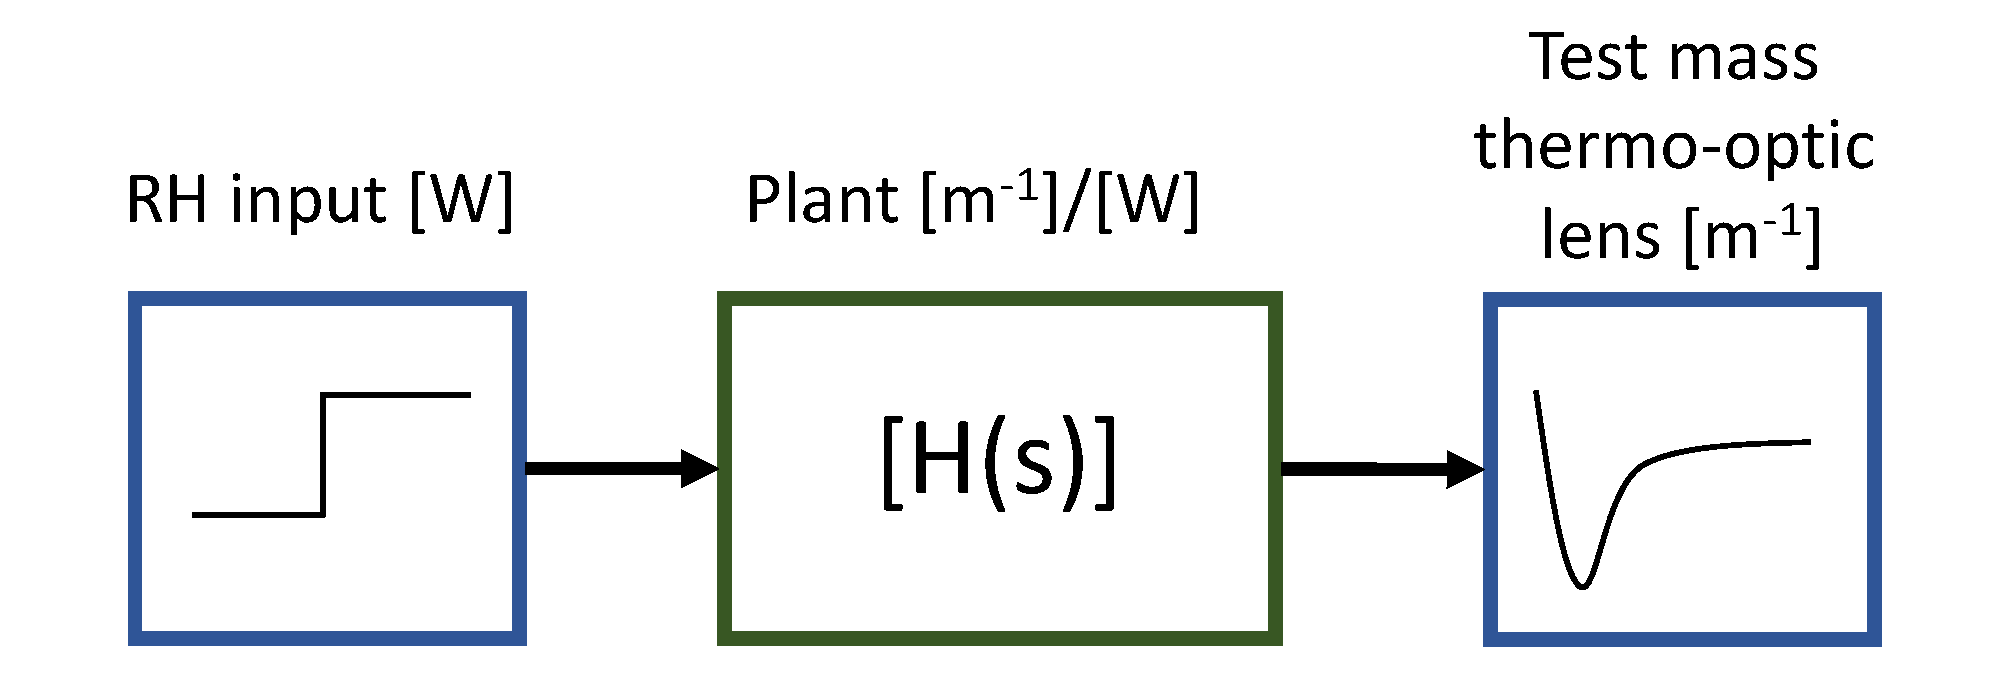
\includegraphics[page=1,width=.75\textwidth]{TCS/IRHF/RH_input_filter_figures.pdf}
\caption{A feedback-style block pictograph of the plant system (test mass mirror and annular ring heater) transforming the ring heater power control step to a time-varying thermo-optic response. The example of this can be seen in Fig [\ref{fig:RHresp}]}
\label{fig:justplant}
\end{figure}

The prescription for creating such a filter is realized through the inversion of the well known step response, alongside additional low passing at high frequency to avoid any control instabilities at high frequency.

\textcolor{red}{see appendix for more detail}
%\begin{enumerate}[label=\arabic*),leftmargin=75pt,nosep]
%	\item Fit step response to a zpk filter $H(s)$ 
%	\item Invert fitted filter ($H(s) \rightarrow H^{-1}(s)$) 
%	\item Apply correction filter $G(s)$ for stability and speed tuning ($H^{-1}(s)*G(s)$)
%\end{enumerate}

\begin{figure}[H]
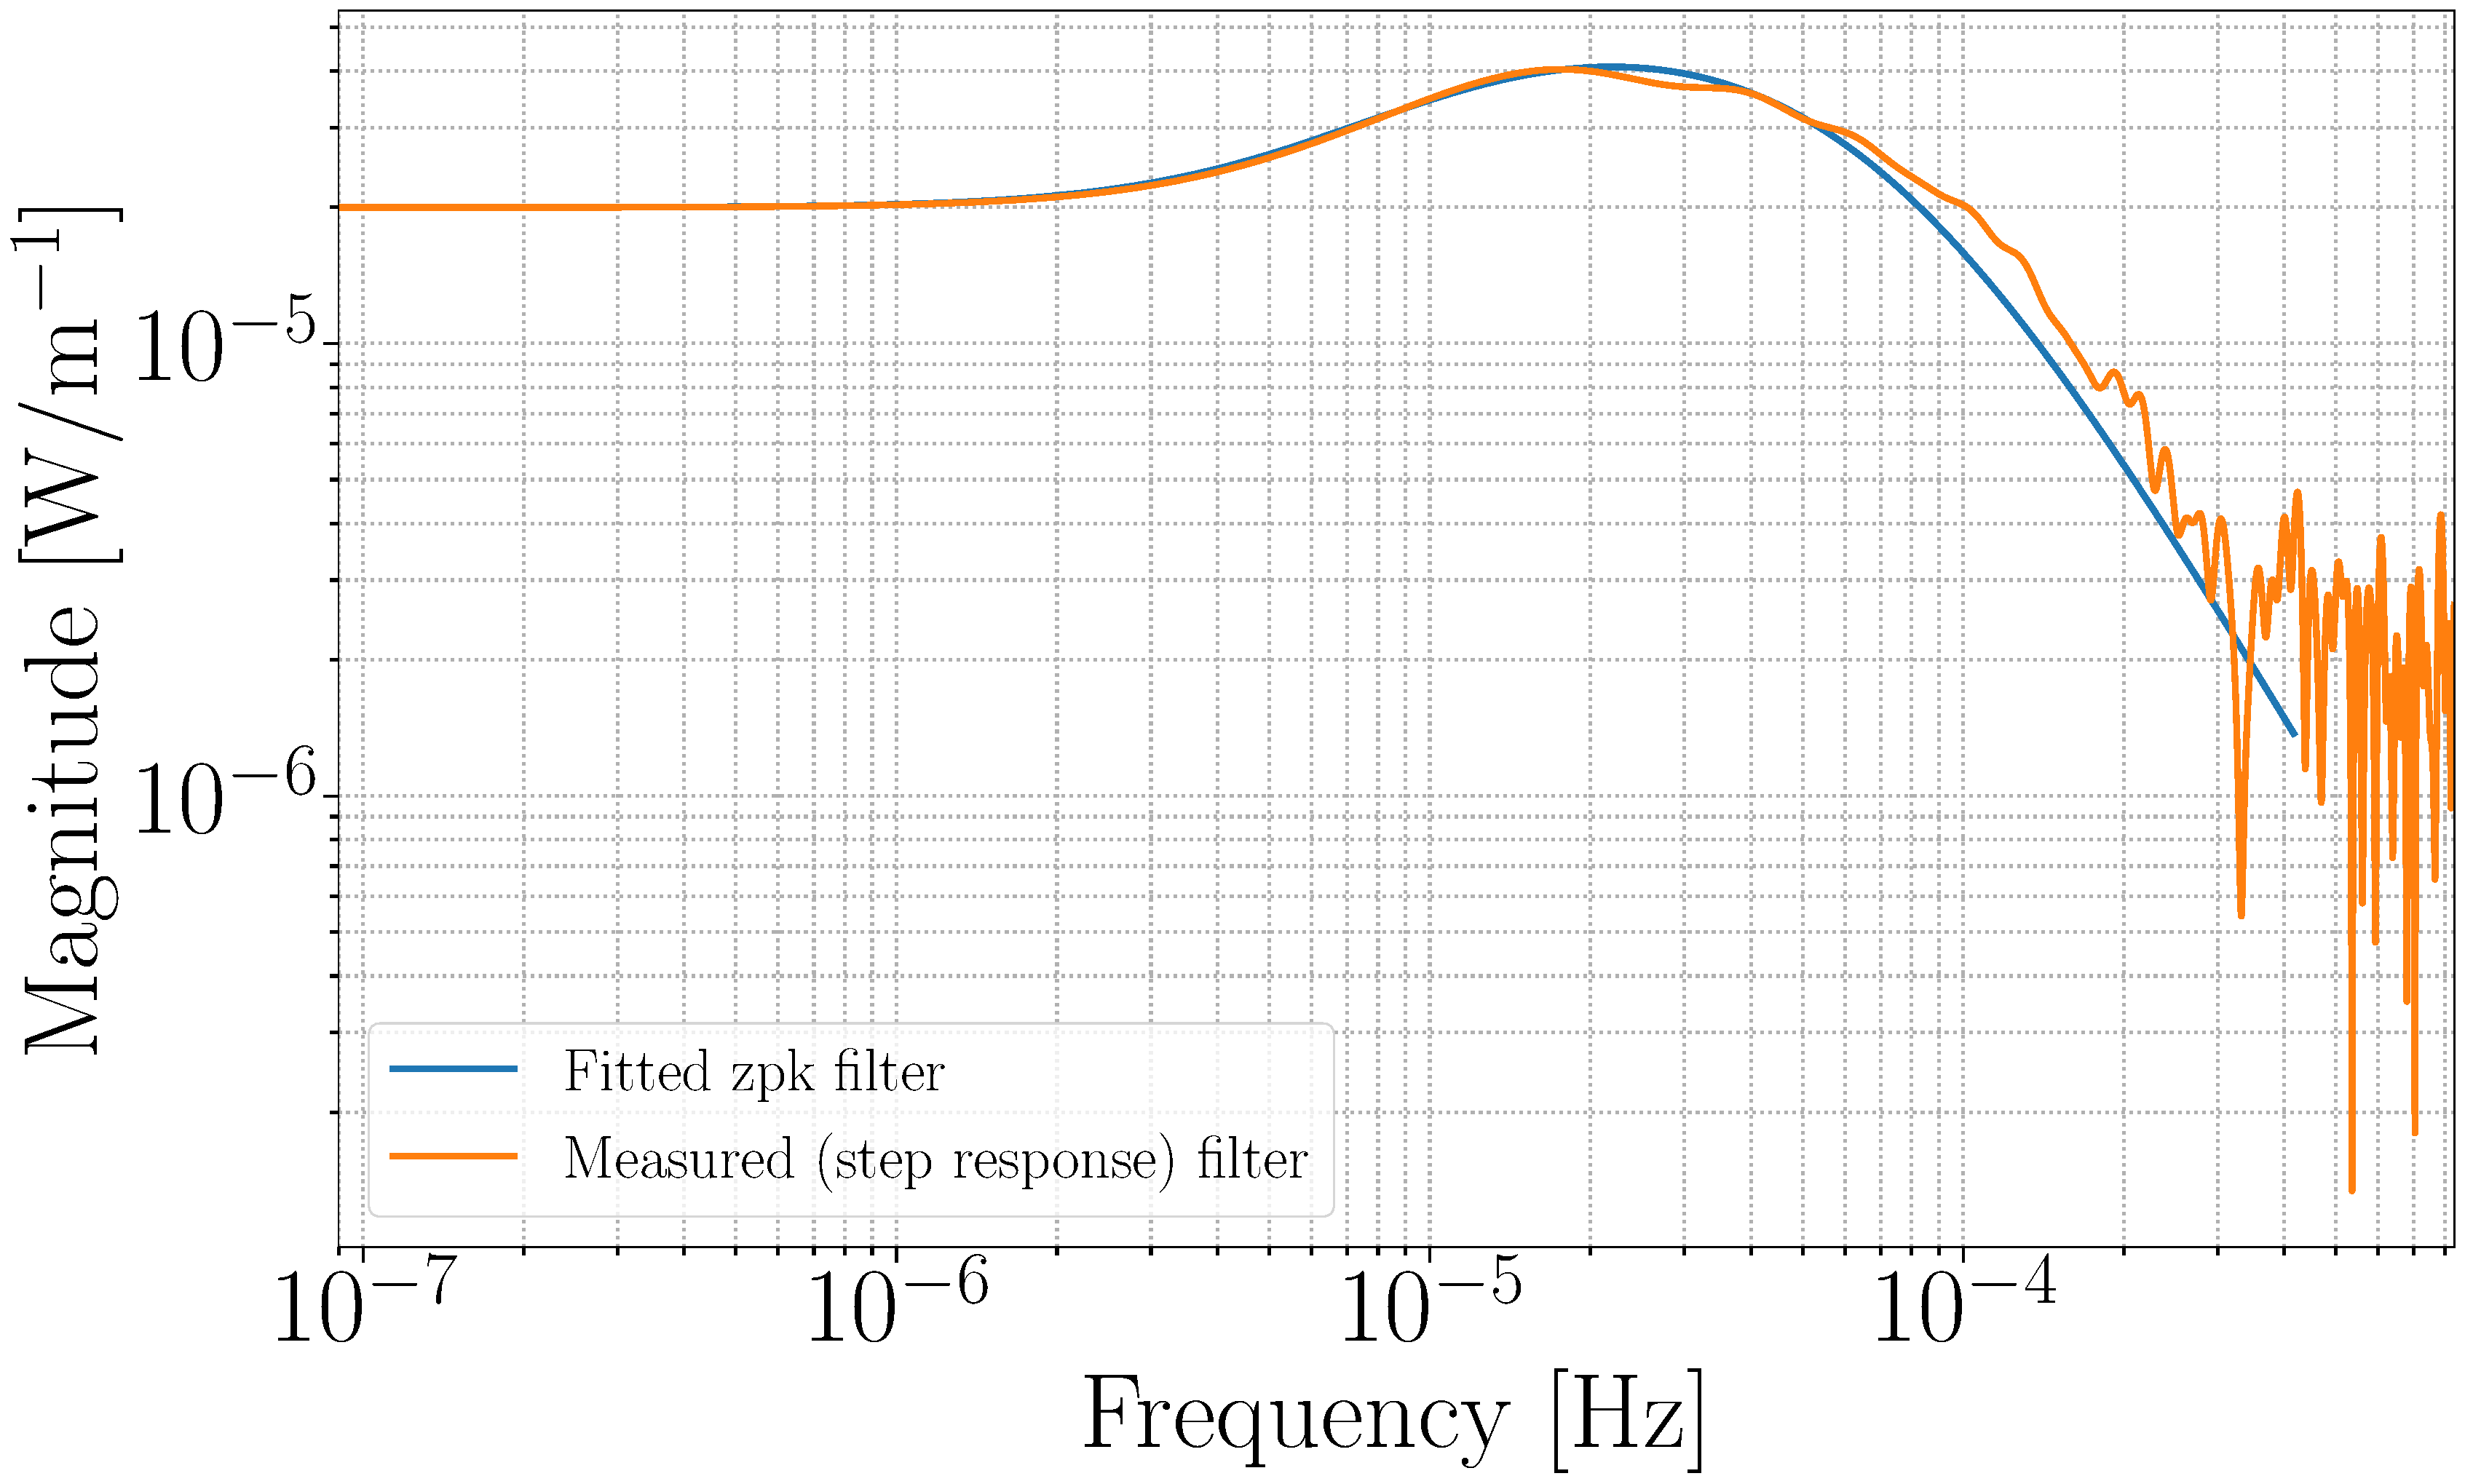
\includegraphics[width=\textwidth]{TCS/IRHF/RH_plant_filter_fit}
\caption{Showing the PSD of the RH response (normalized by the input RH power) over a an $\approx$ 12.5 hour period. The zpk model of the fitted filter (H(s)) is $9.2545e-12 \frac{(s+3.14210e-5)}{(s+8.168e-5)(s+0.0003142)(s+0.0005969)}$}
\label{fig:plant_v_fit}
\end{figure}

\begin{figure}[H]
\centering
\includegraphics[page=2,width=.9\textwidth]{TCS/IRHF/RH_input_filter_figures.pdf}
\caption{A pictograph showing the system with real time digital filtering for an improved thermo-optic response. The RH input filter is created by inverting the plant filter combine with a low pass and added poles to the zpk model to ensure stability.}
\label{fig:rtdf_pictograph}
\end{figure}

\begin{figure}[H]
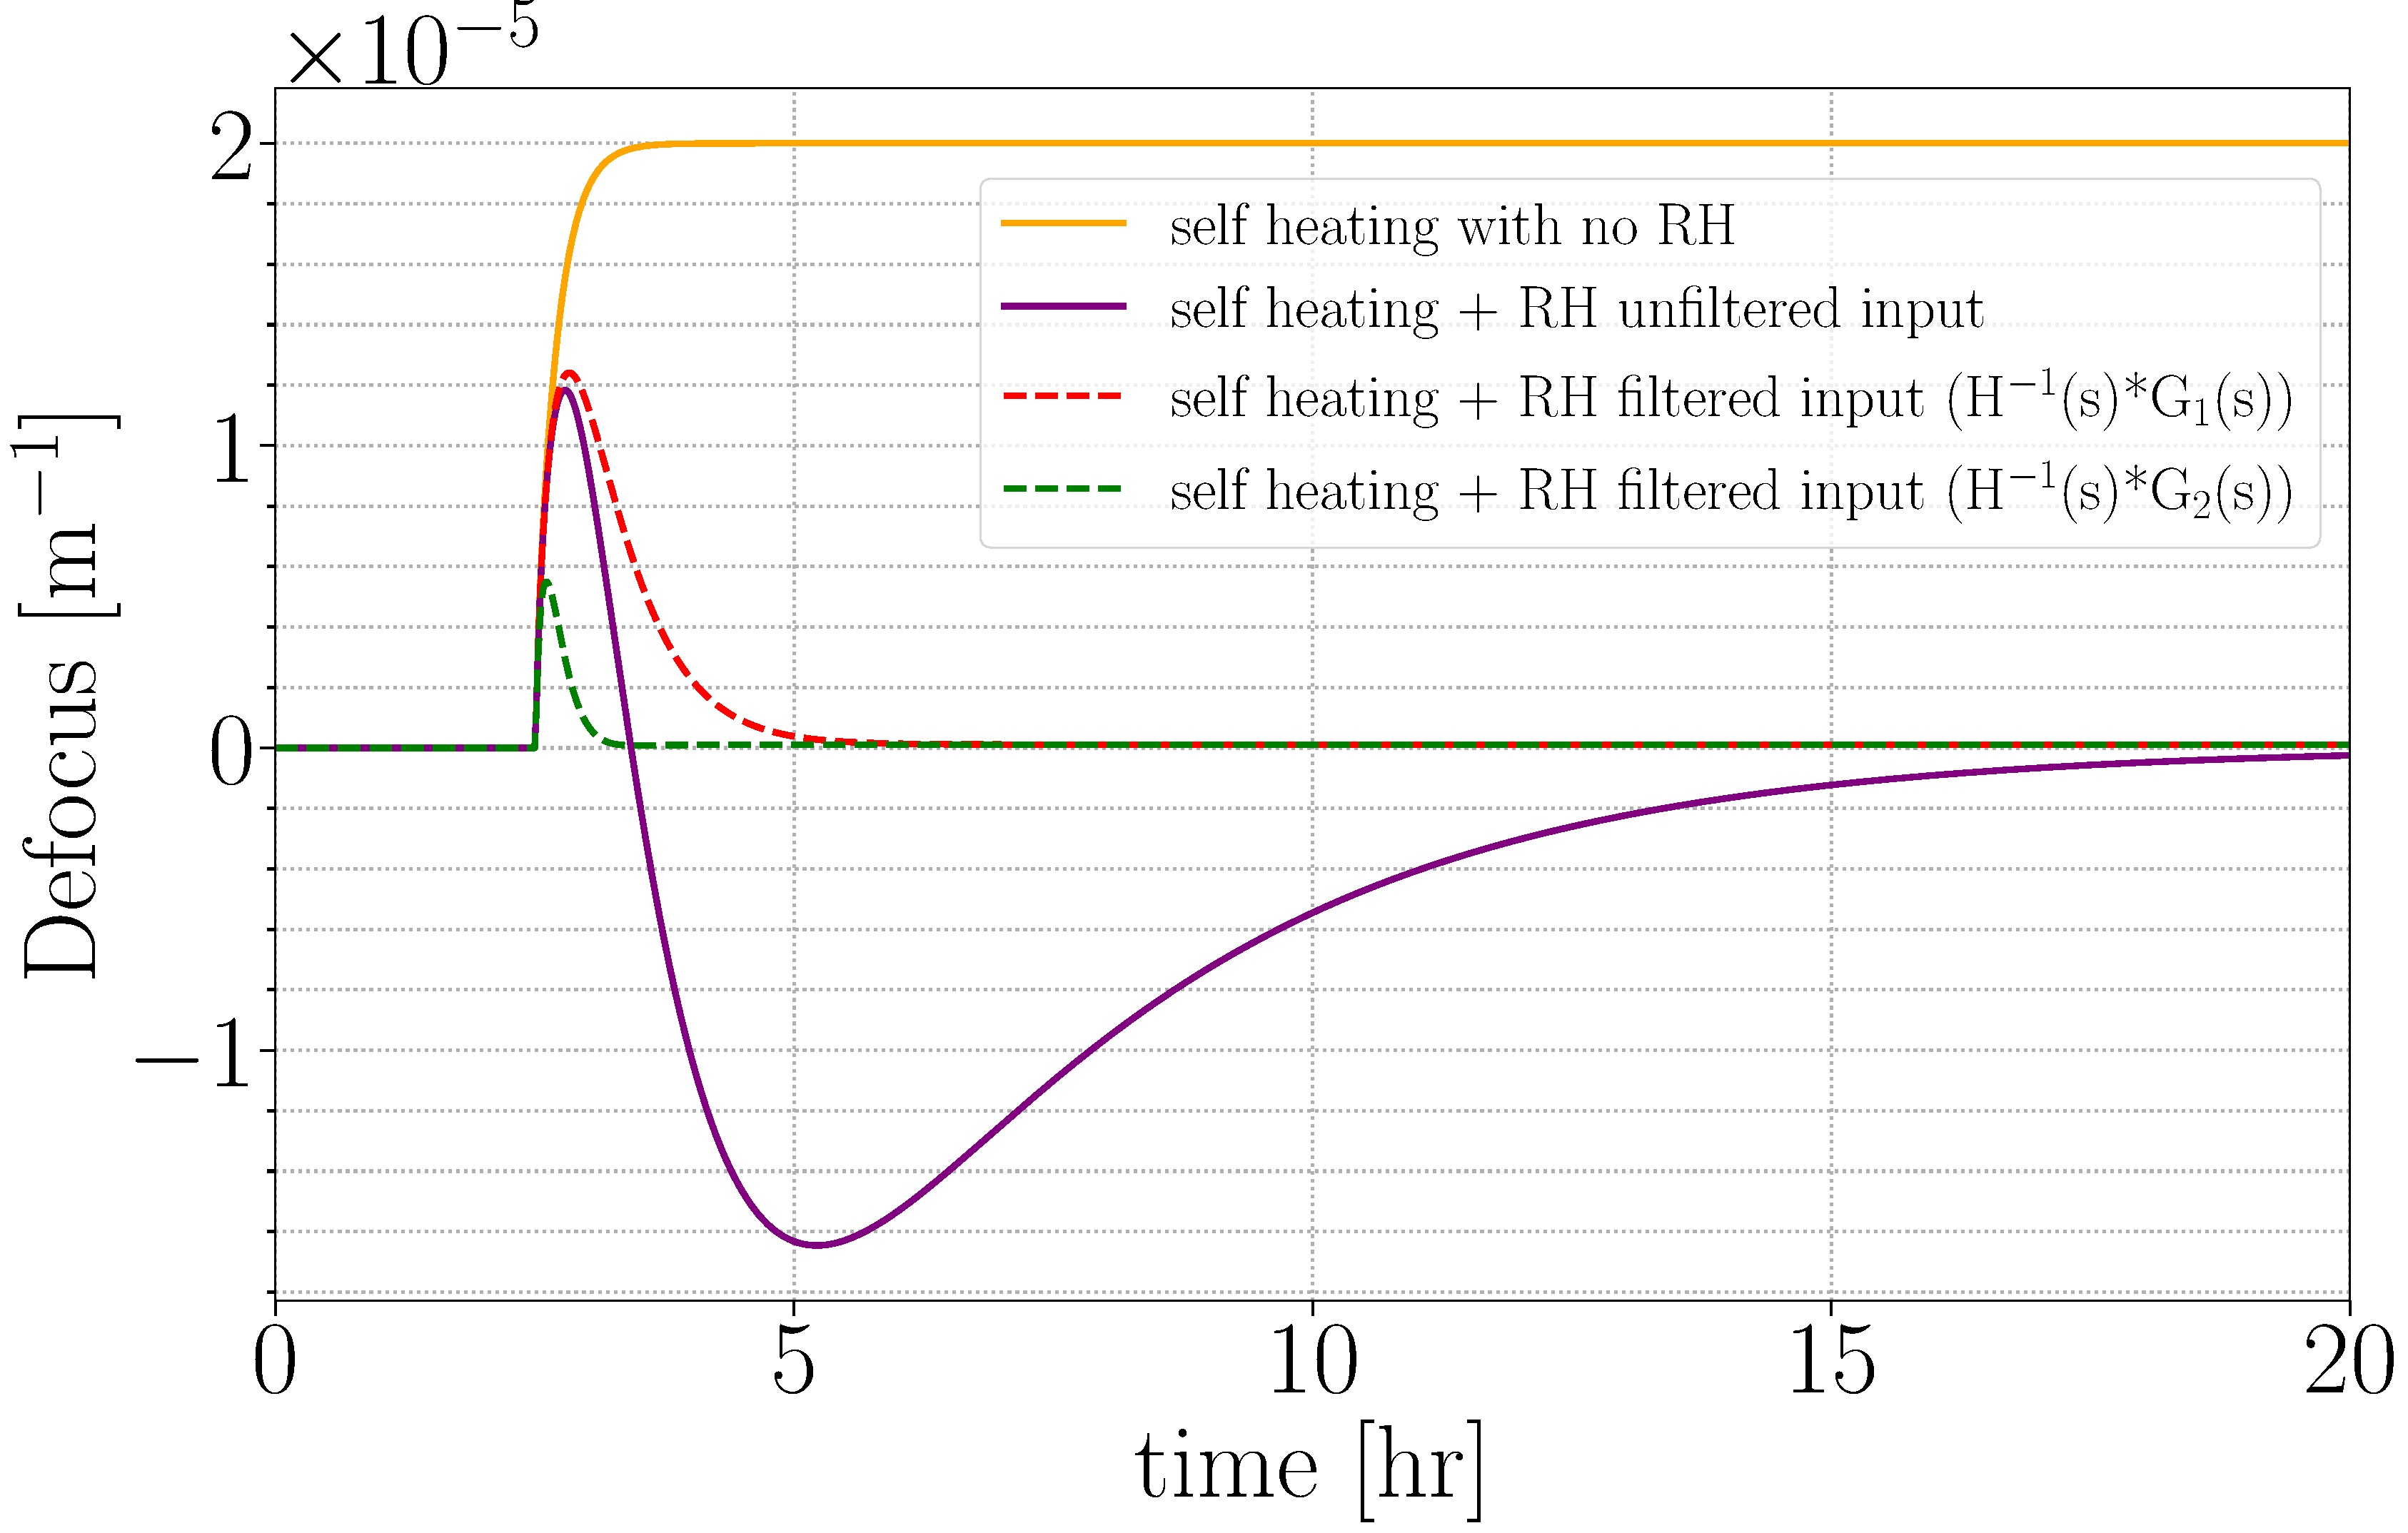
\includegraphics[width=\textwidth]{TCS/IRHF/IRHF_compare_w_self}
\caption{Comparison of the natural RH response and the response to the conditioned input. The above plot is simulated in Matlab by passing the RH input time series (top plot) through the $[H(s)]^{-1*}$ and $H(s)$ to acquire with the result lensing behavior on the bottom plot.}
\label{fig:dynam_comparison}
\end{figure}
\newpage

\subsection{Reducing Parametric Instabilities}
Another symptom of resonant high power optical cavities are parametric instabilities (PI); induced by the opto-mechanical interaction between test mass acoustic modes and higher order optical modes. These PIs present threats to achieving designed detector sensitivity; even driving the detector to lockloss. Passive methods of mitigating PIs by way of acoustic mode dampers (AMD) demonstrate significant reductions of problematic mechanical modes though some (i.e. @ 15 kHz mode) have remained problematic. Lingering parametric instabilities required manual intervention by way of adjusting test mass / cavity geometry to disrupt these persistent PIs, and is now a much more feasible solution with DTC \cite{Hardwick_2020}.  

\subsubsection{Limitations}
\begin{figure}[H]
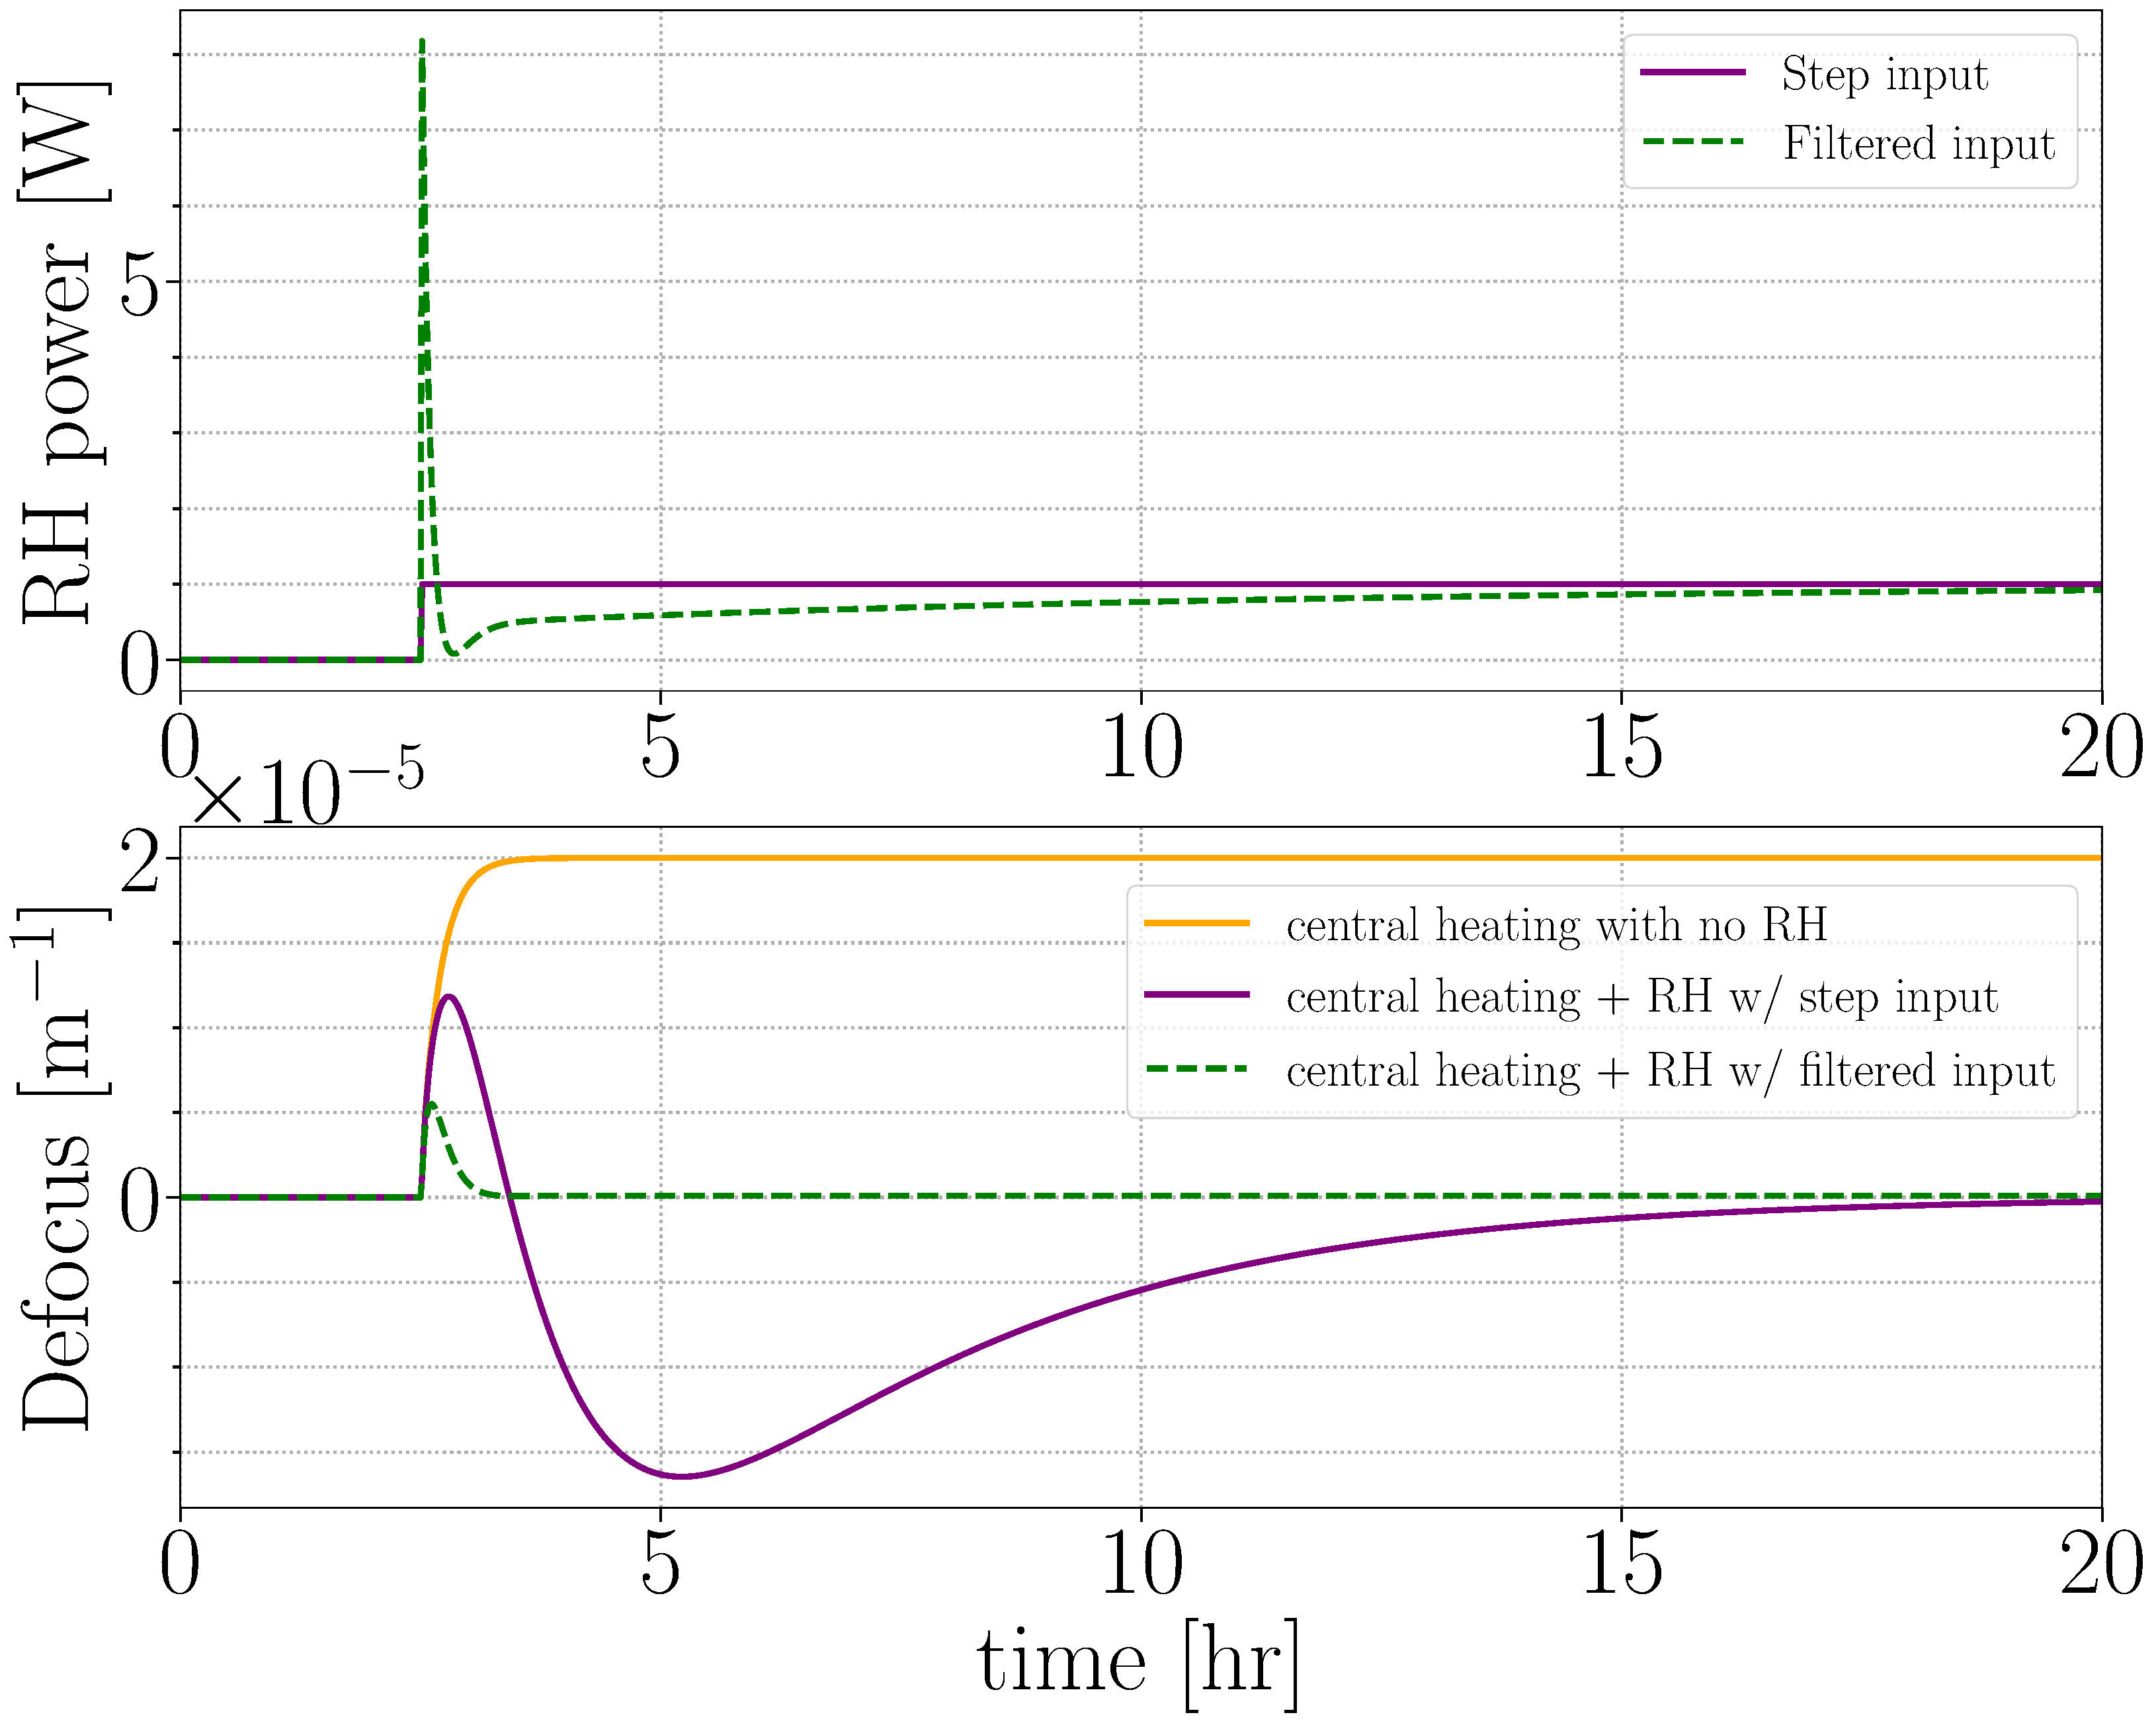
\includegraphics[width=\textwidth]{TCS/IRHF/IRHF_compare_filts_PI_paper}
\caption{Comparison of the natural RH response and the response to the filtered input with RH power}
\label{fig:RH_power}
\end{figure}
Limitation on RH power is set at 8W \textcolor{red}{Double check source?}


